\documentclass[fontsize = 12pt, paper = a4]{scrreprt} 

\setlength{\parindent}{0pt}
\usepackage[english,ngerman]{babel}
\usepackage[utf8]{inputenc}
\usepackage{enumerate}
\usepackage{amssymb,amsmath}

%------------ Überschriften verkleinern und hochsetzen ----------%

\makeatletter
\renewcommand*\@makechapterhead[1]{%
{\parindent \z@ \raggedright \normalfont
\LARGE\bfseries
\ifnum \c@secnumdepth >\m@ne
\thechapter\space
\fi
#1\par\nobreak
\vskip 20\p@
}} 

% ------------------------ Blattlayout- -------------------------%

\usepackage {geometry}   
\geometry   {left     = 2.5cm,
             right    = 2.5cm, 
             top      = 1.5cm,
             bottom   = 1.5cm,
             includehead, includefoot}
             
% ------------------------ Seitenstil ---------------------------%           

% Umdefinieren von Befehlen zur Vermeidung von Bugs:

\renewcommand*{\chapterpagestyle}{scrheadings} 
\renewcommand*{\chapterheadstartvskip}{\vspace*{-\topskip}}

% Gestaltung der Kopf- und Fußzeile:

\pagenumbering{arabic}
            
\usepackage[automark]{scrpage2}
\automark[chapter]{section}
\pagestyle{scrheadings} 
\ohead[\pagemark]{\pagemark}
\setlength{\footskip}{5mm} 

\clearscrheadfoot
\lohead{Entwurfsdokument}
\rohead{\headmark}
\lofoot{Softwareprojekt TU Ilmenau SS 2013}
\rofoot{\pagemark}

% Kopf- und Fußzeilenlinie:

\setheadsepline{.6pt} % Linie für Kopfzeile
\setfootsepline{.6pt} % Linie für Fußzeile 

% Für Unterstreichungen:

\usepackage[normalem]{ulem}

% Buchstabenglättung am Rand:
  
\usepackage {microtype}  

%-------------------------------------------------------------------%

% Für die Einbindung von Bildern:

\usepackage[pdftex]{graphicx} % .pdf, .png oder .jpg möglich!
\usepackage{rotating}         % Grafiken rotieren

% Nutzung in drei Umgebungen möglich:

% (1) \begin{turn}{Winkel} ...  \end{turn}
% (2) \begin{sideways} ... \end{sideways} 90° im math. pos. Sinn
% (3) \begin{rotate}{Winkel} ... \end{rotate} 
%     ---> 90° im math. pos. Sinn, allerdings keine Platzreservierung 

\usepackage{wrapfig}
%\usepackage{picins}   % Textumflossene Grafiken
\usepackage{subfigure}
\usepackage{floatflt}
\usepackage[justification=centering]{caption}

%-------------------------------------------------------------------%
 
% Packete für Tabellen:

\usepackage{booktabs}
\usepackage{array}    % optional
\usepackage{tabularx} % optional

\usepackage[font=footnotesize,labelfont=bf,singlelinecheck=false,
            format=plain,,justification=justified,indention=0cm]                     {caption} 

\usepackage{setspace}

%----------------  Anfang des Dokuments ------------------%

\begin{document}

%*******************************************************************%

% Entwurf Titelseite:

\titlehead{\begin{center}
\textbf{\Huge Entwurfsdokument}
\end{center}}
		   
\title{Service-Interface \\ für ein Formula-Student-Fahrzeug}

\subtitle{Technische Universität Ilmenau \\
		  Softwareprojekt SS 2013 \\ Gruppe 19}			
		
\author{Christian Boxdörfer \\ Thomas Golda \\ Daniel Häger \\ 
		David Kudlek \\  Tom Porzig \\ Tino Tausch \\ 
		Tobias Zehner \\ Sebastian Zehnter}
		
\date{Hier Datum einfügen}	 
	  
\publishers{betreut durch \\ \vspace{1cm} Dr. Heinz-Dietrich Wuttke, TU Ilmenau \\ Oliver Dittrich, fachlicher Betreuer Team StarCraft e.V.}

\maketitle		

%*******************************************************************%

% --------------------- Inhaltsverzeichnis -----------------------%

\begin{spacing}{0.95} 
\tableofcontents
\setcounter{tocdepth}{4} % Anzeige bis Gliederungsstufe 4
\addtocontents{toc}{\protect\enlargethispage{2\baselineskip}} 
\end{spacing}


\newpage % Seitenumbruch

%--------------------------  Einleitung  ---------------------------%

\chapter{Einleitung}

Hier Text einfügen!

%------------------------  Randbedingungen  ------------------------%

\chapter{Randbedingungen} 

Hier Text einfügen!

%--------------------------  Grobentwurf  --------------------------%

\chapter{Grobentwurf}

Hier Text einfügen!

\section{Architekturmuster und Systemzerlegung}
\subsection{dSPACE MicroAutoBox II}
\subsection{Embedded-PC}
\subsection{Webserver}
\subsection{Webseite}
\subsection{Datenbanken}
\subsubsection{Fahrzeugdaten-Datenbank}
\subsubsection{Benutzerdaten-Datenbank}

\section{Simulink-Modell}
\subsection{Verwendete Blöcke}

Um den Einstieg in unsere im folgenden aufgeführte Modellausschnitte  zu erleichtern, werden im Verlauf dieses Abschnittes alle zur Erstellung des Simulink-Modells für die dSPACE MicroAutoBox II verwendeten Blöcke vorgestellt und ihre Funktionsweise kurz erläutert.

\subsubsection{Sources}
\begin{itemize}

\begin{figure}[h]
  \centering
\begin{minipage}[b]{2.5cm}
    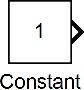
\includegraphics[scale = 0.6]{constant}
    \caption{Constant-Block \label{Constant-Block }}
  \end{minipage}
\hspace*{3cm}  
  \begin{minipage}[b]{5 cm}
    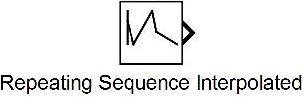
\includegraphics[scale = 0.6]{rsip}
    \caption{Repeating Sequence Interpolated - Block \label{Repeating Sequence Interpolated - Block}}
  \end{minipage}
\end{figure}

\item[1)] \textit{Constant-Block}

%\pichskip{3em}
%\piccaption{Constant-Block \label{Constant-Block}}
%\parpic[r]{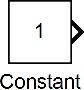
\includegraphics[height = 1.5cm]{constant}}

Der Constant-Block ermöglicht die Generierung eines reellen oder komplexen konstanten Wertes. Je nach Modifikation der Einstellungen 
des Blocks wird es zudem ermöglicht, neben einem konstanten Skalar einen konstanten Vektor oder eine konstante Matrix als Eingangssignal bereitzustellen. Als Datentypen für das Eingangssignal stehen die unter X.Y. aufgeführten Datentypen zur Verfügung.

\item[2)] \textit{"`Repeating-Sequence-Interpolated" \ - Block}

Im Gegensatz zum Costant-Block ermöglicht dieser Block die Erzeugung eines individuellen, sich periodisch wiederholenden und kontinuierlichen Signals mittels einer Interpolation anhand zuvor selbst definierter diskreter Zeit- und Funktionswerte, welche in zwei Vektoren gleicher Länge gespeichert sind.

\end{itemize}

%\newpage

\subsubsection{Ports \& Subsystems}

\begin{itemize}

\begin{figure}[h]
  \centering
  \begin{minipage}[b]{2.5 cm}
    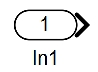
\includegraphics[scale = 0.6]{inport}
    \caption{Inport-Block \label{Inport}}
  \end{minipage}
  \hfill
  \begin{minipage}[b]{2.5 cm}
    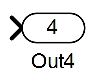
\includegraphics[scale = 0.6]{outport}
    \caption{Outport-Block \label{Outport}}
  \end{minipage}
  \hfill
  \begin{minipage}[b]{3.5 cm}
    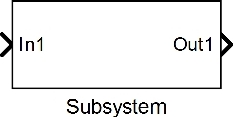
\includegraphics[scale = 0.5]{subsystem}
    \caption{Subsystem \label{Subsystem}}
  \end{minipage}  
\end{figure}


\item[1)] \textit{Inport-Block}

Dieser Block hat in unserem Modell die Aufgabe, die zuvor festgelegten Eingangssignale des Subsystems auf der Modellebene des Subsystems selbst zu repräsentieren. Darüber hinaus mit ist es in der Top-Level-Ebene des Systems mit diesem Block auch möglich, externe Eingangssignale aus dem Arbeitsbereich für das Modell bereitzustellen. 

\item[2)] \textit{Outport-Block}

Die Aufgabe des Outport-Blockes ist es, eine Verknüpfung vom aktuellen System zu einem Zielsystem außerhalb der Modellebene herzustellen.

\item[3)] \textit{Subsystem}

Innerhalb eines Subsystems können verschiedene Blöcke zusammengefasst werden, was eine Strukturierung und Gliederung der Signalflüsse erleichtert und zudem eine deutlich übersichtlichere Darstellung des Modells zur Folge hat. Weiterhin ist es auch möglich, mehrere Subsysteme in einem Subsystem zusammenzufassen, um eine beliebige Tiefe innerhalb der Hierarchie eines Modells zu realisieren. 

%\newpage  

\end{itemize}

\subsubsection{Signal Routing}

\begin{itemize}

\begin{figure}[h]
\centering
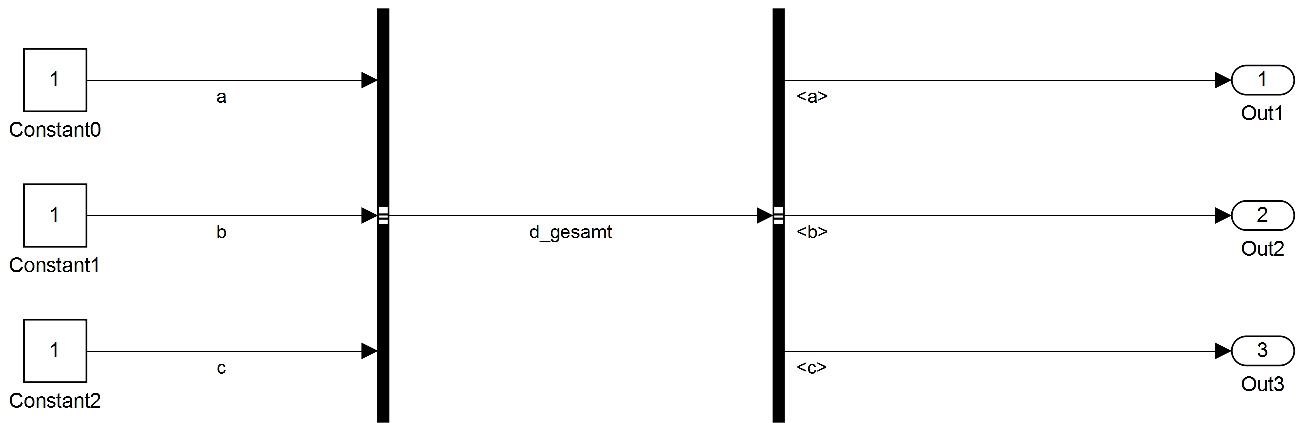
\includegraphics[scale = 0.45]{bus_gesamt}
\caption{Bussystem bestehend aus einem Bus Creator (l.) und einem Bus Selector (r.)}
\end{figure}


\item[1)] \textit{Bus Creator}

Mit Hilfe eines solchen Bus Creators wird es ermöglicht, mehrere Signale (a, b, c) zu einem Gesamtsignal (d\_gesamt) zu bündeln.

\item[2)] \textit{Bus Selector}

Umgekehrt erlaubt es der Bus Selector, aus einem Gesamtsignal wieder einzelne Signale zu selektieren und diese gesondert weiterzuleiten. So wird wie in Abb. X.Y. dargestellt wieder aus dem Gesamtsignal d\_gesamt die Signale a, b und c herausgeführt.

\end{itemize}

\subsubsection{Signal Attributes}

\begin{itemize}

\begin{figure}[h]
  \centering
\begin{minipage}[b]{2.5cm}
    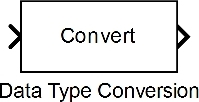
\includegraphics[scale = 0.5]{convert}
    \caption{Convert-Block \label{Convert-Block}}
  \end{minipage}
\hspace*{3cm}  
  \begin{minipage}[b]{5 cm}
    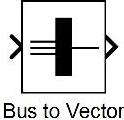
\includegraphics[scale = 0.5]{bustovector}
    \caption{Bus to Vector - Block \label{Bus to Vector - Block}}
  \end{minipage}
\end{figure}

\item[1)] \textit{Convert-Block}

Mit dem Convert-Block können verschiedene Anforderungen realisiert werden:

\begin{itemize}
\item Konvertierung eines Signals bzw. eines Signalvektors in einen anderen Datentyp, hierbei kann die Art der Rundung selbst festgelegt werden.

\item Umbenennung eines Signals bzw. eines Signalvektors. \\
Dies hat den Zweck, dass man nach dem Convert-Block unabhängig vom  angelegten Eingangssignal mit einem festen Datentyp und einem fest vergebenem Variablennamen in anderen Systemen bzw. auf anderen Plattformen arbeiten kann.  

\end{itemize} 

\item[2)] \textit{"`Bus to Vector"\ - Block}

Dieser Block konvertiert ein virtuelles Bussignal in ein Vektorsignal. Hierbei ist es erforderlich, dass alle am zu konvertierenden Bus anliegenden Signale im Datentyp, Signaltyp und im gewählten Sampling-Verfahren übereinstimmen.

\end{itemize}

\subsubsection{Sinks}

\begin{itemize}

\begin{figure}[h]
  \centering
  \begin{minipage}[b]{2.75 cm}
    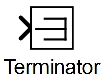
\includegraphics[scale = 0.6]{terminator}
    \caption{Terminator-Block \label{Terminator-Block}}
  \end{minipage}
  \hfill
  \begin{minipage}[b]{2.5 cm}
    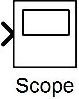
\includegraphics[scale = 0.6]{scope}
    \caption{Scope \label{Scope}}
  \end{minipage}
  \hfill
  \begin{minipage}[b]{3.5 cm}
    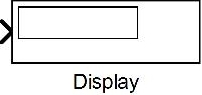
\includegraphics[scale = 0.6]{display}
    \caption{Display \label{Display}}
  \end{minipage}  
\end{figure}


\item[1)] \textit{Terminator}

Der Terminator dient dazu, die Signale, deren Ausgänge nicht mit Blöcken o.ä. verbunden sind, abzuschließen. 

\item[2)] \textit{Scope}

Der Scope-Block stellt den Signalverlauf eines Signals über der Simulationszeit dar, weswegen er sich hervorragend dafür eignet ein erstelltes Modell auf dessen Korrektheit zu überprüfen.

\item[3)] \textit{Display}

Der Display-Block zeigt den konkreten Wert eines Eingangssignals an. Um die Anzeige des Displays anzupassen, kann der Entwickler über die Einstellungen der Format-Parameter Einfluss darauf nehmen.  

\end{itemize}

\subsubsection{Math Operations}

\begin{itemize}

\item[1)] \textit{Gain-Block}

Der Gain-Block multipliziert das Eingangssignal mit einer selbst gewählten Konstante, wobei das Eingangssignal selbst ein Skalar, ein Vektor oder eine Matrix sein kann.


\end{itemize}

\subsubsection{dSPACE-Blöcke}

Im Folgenden sollen nun diejenigen Blöcke vorgestellt werden, welche speziell für eine Verwendung mit der MicroAutoBox II konzipiert wurden und u.a. für eine Kommunikation ebendieser mit dem Embedded-PC unerlässlich sind. 

\begin{itemize}

\item[1)] \textit{Encode32-Block}

\item[2)] \textit{"`UDP Send" \ - Block} 

\end{itemize}

\subsection{Signalgenerator}

Das Modell, welches auf der dSPACE MicroAutoBox II implementiert wird, besitzt zwei Subsysteme - den Signalgenerator und den Signalkollektor. Der Signalgenerator hat hierbei die Aufgabe, auf der MicroAutoBox II die für einen Systemtest benötigten Testsignale zu generieren, welche anschließend zum Embedded-PC via UDP-Schnittstelle gelangen und daraufhin per GPRS / UMTS an einen vServer gesendet werden. Dieses Subsystem wird jedoch nach einem erfolgreichen Test des Service-Interfaces durch ein Subsystem von Team Starcraft e.V. ersetzt, welches im Stande ist die im Formula-Student-Fahrzeug verbauten Komponenten anzusprechen und somit im Unterschied zu dem aktuell verwendeten Signalgenerator statt künstlich erzeugter Daten die realen Daten auszulesen und an den Signalkollektor weiterzuleiten.   

\subsubsection{Struktur des Subsystems}

Um ein hohes Maß an Übersichtlichkeit und Modularität zu gewährleisten, wird an den Vorgaben von Team StarCraft e.V. orientierend das Subsystem des Signalgenerators nochmals in einzelne Subsysteme unterteilt, die die verschieden Kategorien der jeweiligen Fahrzeugdaten repräsentieren. 

\begin{figure}[h]
\centering
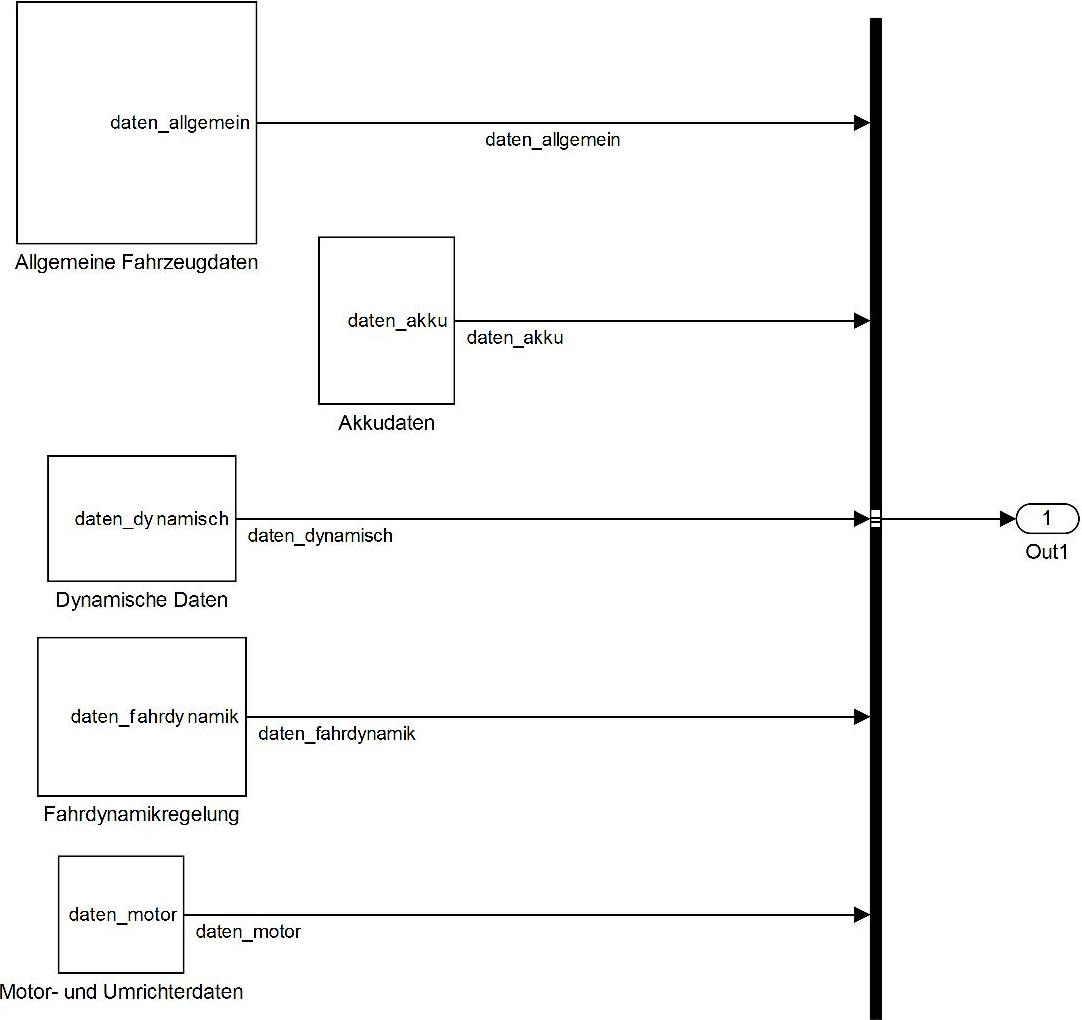
\includegraphics[scale = 0.8]{signalgen}
\caption{Subsysteme des Signalgenerators nach den Kategorien der Fahrzeugdaten}
\end{figure}

Innerhalb dieser Subsysteme findet nun - ohne Beschränkung der Allgemeinheit am Subsystem "`Daten Allgemein"\ erläutert - die Signalerzeugung (Geschwindigkeit, Gesamtspannung des Akkus und der Fahrzeugzeit) statt, wobei wie in X.Y dargestellt die Signalerzeugung mehrere Signale der gleichen "`Signalgruppe"\ wiederum zu Subsystemen (Notausfunktionen, Temperaturen und Gaswerte)  innerhalb des Subsystems "`Allgemeine Daten"\ zusammengefasst werden. Die eigentliche Erzeugung der Signale wird wie in Abbildung X.Y. gezeigt mittels Blöcken aus der Kategorie "`Sources" (s. X.Y) realisiert. Hierbei wird je nach Input entweder ein Constant-Block mit dem Datentyp \textit{boolean} zur Realisierung von Schaltern etc. (s. Notausfunktionen)oder ein Repeating Sequence Interpolated (RSI) - Block mit dem Datentyp \textit{single} zur Modellierung der restlichen Fahrzeugkomponenten verwendet (s. Gaswerte). Der Datentyp \textit{single} wurde deshalb gewählt, um auch wie von Team StarCraft e.V. gefordert als Input Werte mit mehreren Nachkommastellen realisieren zu können. Die auf analoge Weise zu X.Y mit Constant- oder RSI-Blöcken erzeugten 386 Input-Signale werden schließlich im Umkehrschluss zur obigen Beschreibung über mehrere Bussysteme und Subsysteme zu einem Busarray im Signalgenerator zusammengefasst, welcher nunmehr dieses an den Signalkollektor übergibt.   

%\newpage



\begin{figure}[h]
\centering
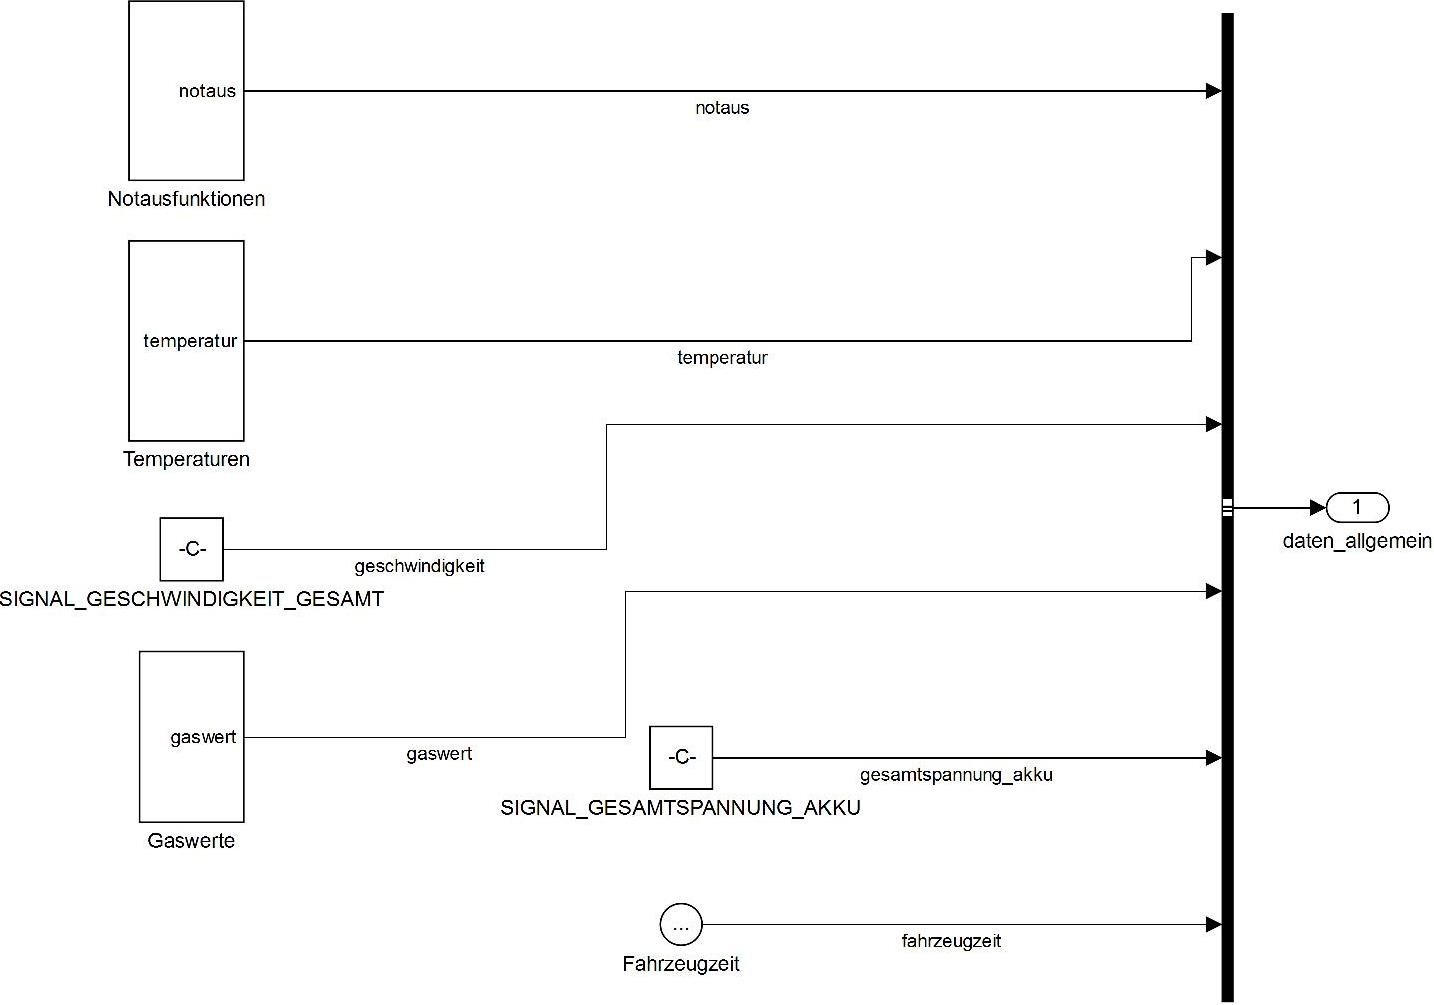
\includegraphics[scale = 0.65]{suballgemein}
\caption{Subsystem "`Allgemeine Daten"\ im Signalgenerator}
\end{figure}
  
\begin{figure}[h]
\centering
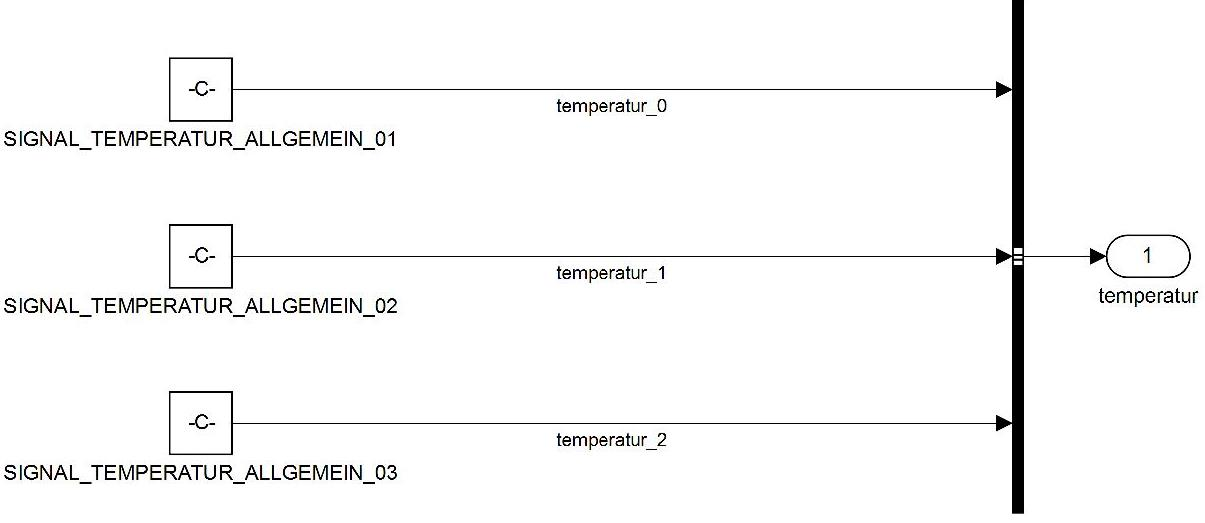
\includegraphics[scale = 0.65]{subsubtemp}
\caption{Signalerzeugung im Subsystem "'Temperaturen"}
\end{figure}


\subsubsection{Config-Datei "`signalgenerator\_microautobox.m" }

Um eine mögliche Änderung der Testsignale zu vereinfachen und eine übersichtliche Darstellung aller Testsignale zu realisieren, sorgt eine Konfigurationsdatei in Matlab für die Spezifizierung der Testsignale des Simulink-Modells. Die in dem *.m-File aufgeführten Parameter für die Zeit- und Funktionsvektoren dienen als Referenz für die signalerzeugenden Blöcke, welche über den Workspace von Matlab auf diese nach dem Ausführen der Datei zugreifen können (s. Abb. X.Y). Hierbei sollte jedoch beachtet werden, dass vor dem Compilieren des Simulink-Modells und der Implementierung ebendiesem auf der MicroAutoBox II einmalig das *.m-File ausgeführt werden muss. Demzufolge muss auch nach dem Ändern von Parametern die Datei neu ausgeführt werden, damit bei einer erneuten Implementierung des Simulink-Modells die geänderten Parameter korrekt übernommen werden können. Zudem wurde auch um die Benennung der Parameter im *.m-File zu standardisieren jeder Funktionsvektor mit dem Präfix "`SIGNAL\_"\ und jeder Zeitvektor mit dem Präfix "`TIME\_"\ versehen. 

\begin{figure}[h]
\centering
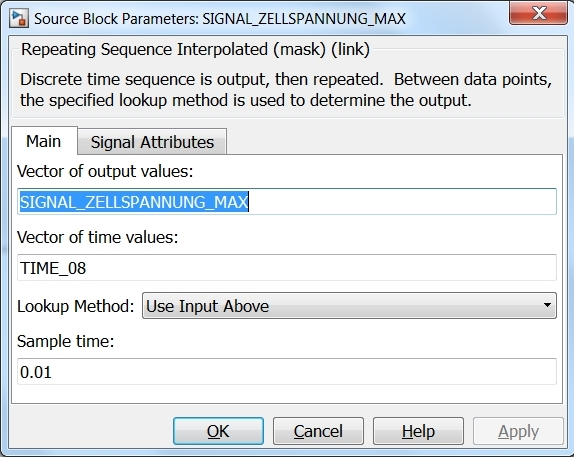
\includegraphics[scale = 0.75]{referenz}
\caption{Referenzierung im RSI-Block}
\end{figure}


\subsection{Signalkollektor}

Der Signalkollektor stellt wie bereits erwähnt das zweite große Subsystem innerhalb des Simulink-Modells dar. Er hat die Aufgabe den vom Subsystem "`Signalgenerator"\ (s. X.Y) oder von einem späteren Subsystem von Team StarCraft e.V. erhaltenen Busarray wieder in die einzelnen Signale zu unterteilen, ggf. geeignet aufzubereiten und diese dann eine UDP-Schnittstelle innerhalb des Subsystems weiterzuleiten, welche die erzeugten Testsignale bzw. Testdaten an den Embedded-PC sendet.  

\subsubsection{Struktur des Subsystems}

Das Subsystem selbst besitzt die folgende innere Struktur: \\
In einem ersten Schritt wird das Busarray wieder in den Kategorien A) - E) der Fahrzeugdaten entsprechenden Signalgruppen aufgeteilt und den fünf Subsystemen (vgl. Abb. X.Y) zugeführt. Dort werden die nunmehr fünf Busarrays wieder über mehrere Busselektoren und Subsysteme hinweg in die 368 einzelnen Signale aufgelöst, welche somit einzeln aufbereitet werden können (s. Abb. X.Y). Während der Aufbereitung der Signale werden die folgenden Schritte durchgeführt:

\begin{figure}[h]
\centering
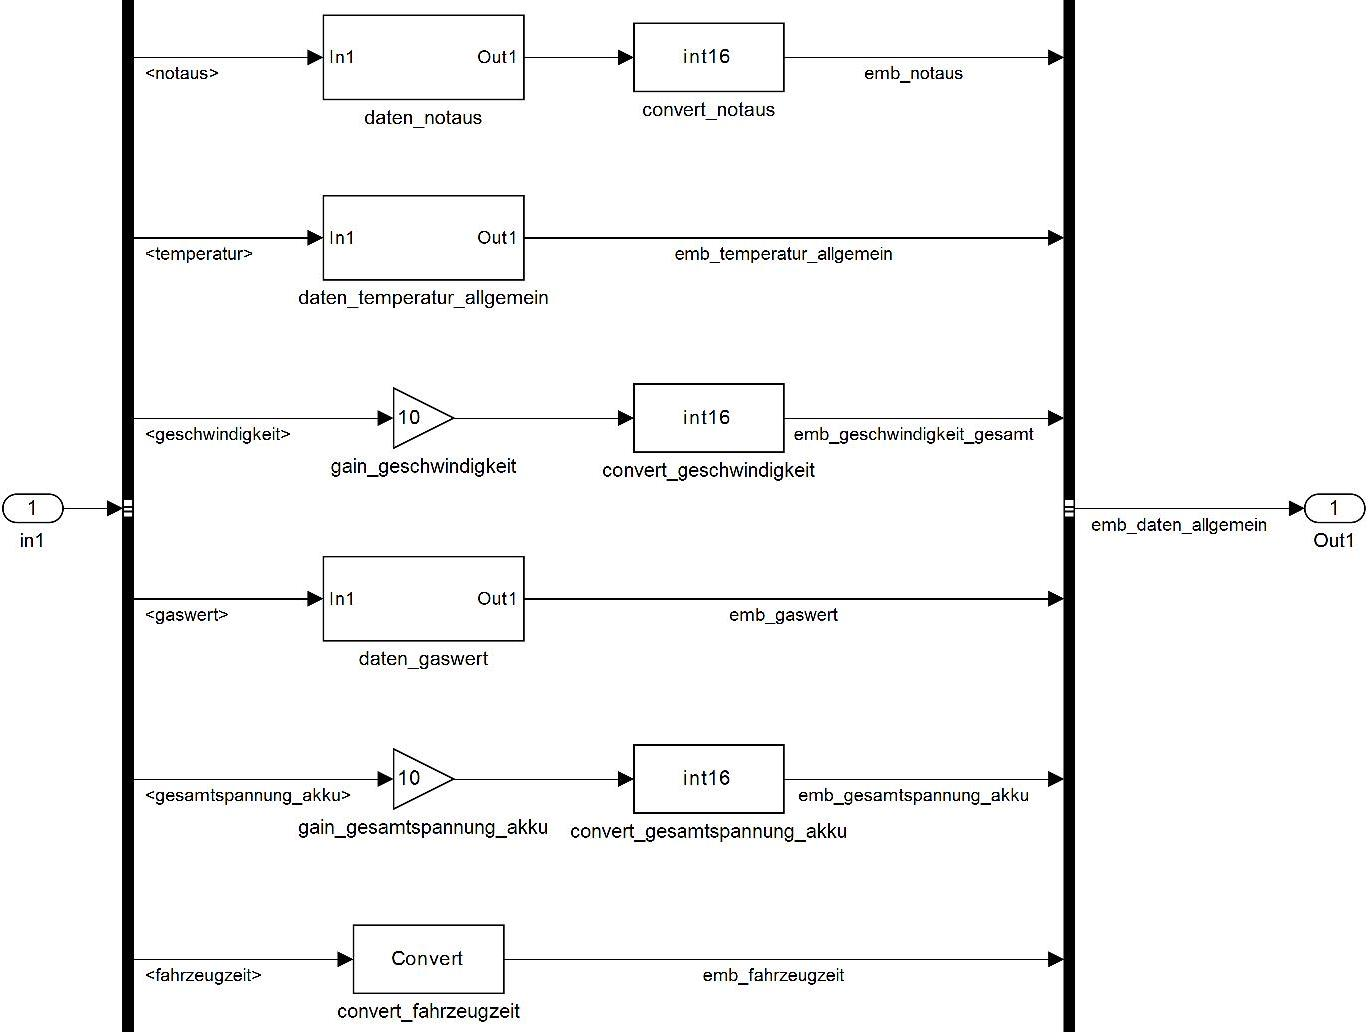
\includegraphics[scale = 0.70]{collallgemein}
\caption{Signalaufbereitung im Subsystem "`daten\_allgemein"}
\end{figure} 


\begin{itemize}

\item[1)] \textit{Verstärkung der Signale}

Abhängig von der Anzahl der Nachkommastellen des Testsignals $n\ mit\ n>0$ wird dieses nun durch einen Gain-Block (s. X.Y) mit dem Faktor $10^n$ multipliziert, um für den aktuellen Wert des Testsignals jeweils einen ganzzahligen Wert zu erhalten, was zur Vereinheitlichung der zu übertragenden Daten beiträgt.

\item[2)] \textit{Konvertierung der Datentypen}

Die nunmehr ganzzahligen Werte werden von ihren Datentypen \textit{boolean} oder \textit{single} nun einheitlich mittels eines Convert-Blocks (s. X.Y) in den Datentyp \textit{int16} konvertiert, wodurch somit alle Signale den gleichen Datentyp aufweisen.  

\item[3)] \textit{Umbenennung der Variablennamen}

Mit dem Convert-Block ist es zudem möglich, dem Ausgangssignal unabhängig vom Eingangssignal einen festen bzw. neuen Variablennamen zu vergeben. Dies ist insofern nützlich, da bei einem möglichen Zugriff auf die Daten bzw. die Variablen durch den Embedded-PC diese immer die gleichen Variablennamen besitzen, unabhängig davon ob der Signalgenerator durch das Subsystem von Team StarCraft e.V. ersetzt wurde oder nicht.

\end{itemize}  

Nachdem die Daten anhand der obigen Schritte aufbereitet wurden, werden dieser erneut durch mehrere Bus Creator und Subsysteme auf einem zentralen Bus Creator zu einem Busarray gebündelt und auf einen Bus to Vector - Block (s. X.Y.) gegeben, welcher das Busarray in einen Vektor umwandelt. Anschließend wird dieser Vektor der UDP-Schnittstelle zugeführt.


\subsection{UDP-Schnittstelle}




%--------------------------  Feinentwurf  --------------------------%

\chapter{Feinentwurf} 

%---------------------------  Glossar  -----------------------------%

\chapter*{Glossar}

%----------------------  Abbildungsverzeichnis  --------------------%

%\chapter*{Abbildungsverzeichnis}

\listoffigures
%
%---------------------------  Anhang  ------------------------------%

\chapter*{Anhang}

%\textbf{Datentypen in Simulink}
%
%\begin{itemize}
%
%\item xd
%
%\end{itemize}



\end{document}